\documentclass[border=10pt]{standalone}
\usepackage{pgfplots}
\pgfplotsset{compat=1.18}
\begin{document}
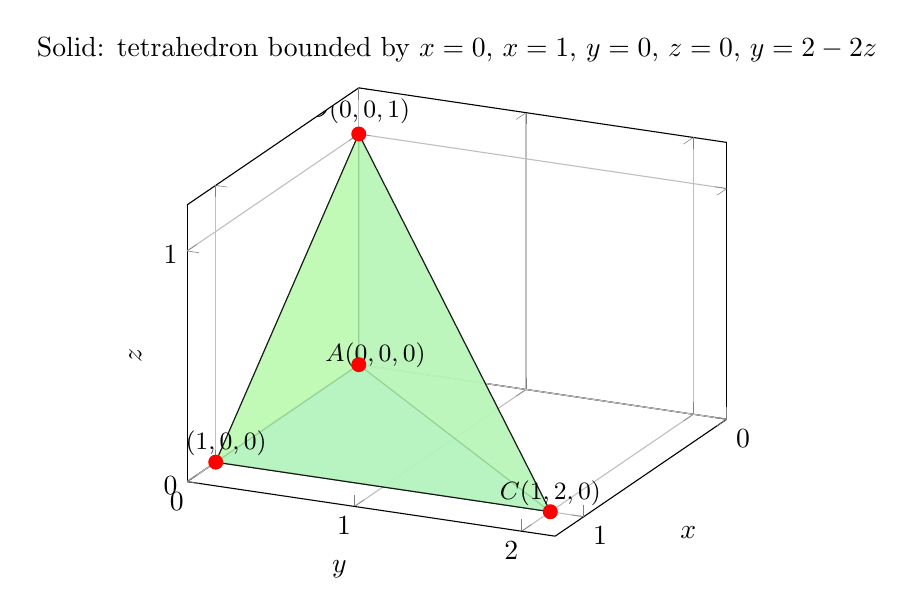
\begin{tikzpicture}
\begin{axis}[
    view={115}{25},
    xlabel={$x$}, ylabel={$y$}, zlabel={$z$},
    xmin=0, xmax=1.2, ymin=0, ymax=2.2, zmin=0, zmax=1.2,
    xtick={0,1}, ytick={0,1,2}, ztick={0,1},
    grid=major,
    title={Solid: tetrahedron bounded by $x=0$, $x=1$, $y=0$, $z=0$, $y=2-2z$},
]
% bottom face z=0: A(0,0,0), B(1,0,0), C(1,2,0)
\addplot3[fill=blue!30, opacity=0.7, draw=black] coordinates {(0,0,0) (1,0,0) (1,2,0) (0,0,0)};
% side face y=0: A(0,0,0), B(1,0,0), D(0,0,1)
\addplot3[fill=orange!30, opacity=0.7, draw=black] coordinates {(0,0,0) (1,0,0) (0,0,1) (0,0,0)};
% side face x=0: A(0,0,0), C(1,2,0), D(0,0,1)
\addplot3[fill=violet!25, opacity=0.7, draw=black] coordinates {(0,0,0) (1,2,0) (0,0,1) (0,0,0)};
% slanted face y = 2-2z: B(1,0,0), C(1,2,0), D(0,0,1)
\addplot3[fill=green!30, opacity=0.8, draw=black] coordinates {(1,0,0) (1,2,0) (0,0,1) (1,0,0)};
% vertices
\addplot3[only marks, mark=*, mark size=2.5pt, color=red] coordinates {(0,0,0) (1,0,0) (1,2,0) (0,0,1)};
\node at (axis cs:0,0.1,0.05) {\small $A(0,0,0)$};
\node at (axis cs:1,0,0.08) {\small $B(1,0,0)$};
\node at (axis cs:1,2,0.08) {\small $C(1,2,0)$};
\node at (axis cs:0,0,1.1) {\small $D(0,0,1)$};
\end{axis}
\end{tikzpicture}
\end{document}